% Options for packages loaded elsewhere
\PassOptionsToPackage{unicode}{hyperref}
\PassOptionsToPackage{hyphens}{url}
%
\documentclass[
]{article}
\usepackage{amsmath,amssymb}
\usepackage{lmodern}
\usepackage{iftex}
\ifPDFTeX
  \usepackage[T1]{fontenc}
  \usepackage[utf8]{inputenc}
  \usepackage{textcomp} % provide euro and other symbols
\else % if luatex or xetex
  \usepackage{unicode-math}
  \defaultfontfeatures{Scale=MatchLowercase}
  \defaultfontfeatures[\rmfamily]{Ligatures=TeX,Scale=1}
\fi
% Use upquote if available, for straight quotes in verbatim environments
\IfFileExists{upquote.sty}{\usepackage{upquote}}{}
\IfFileExists{microtype.sty}{% use microtype if available
  \usepackage[]{microtype}
  \UseMicrotypeSet[protrusion]{basicmath} % disable protrusion for tt fonts
}{}
\makeatletter
\@ifundefined{KOMAClassName}{% if non-KOMA class
  \IfFileExists{parskip.sty}{%
    \usepackage{parskip}
  }{% else
    \setlength{\parindent}{0pt}
    \setlength{\parskip}{6pt plus 2pt minus 1pt}}
}{% if KOMA class
  \KOMAoptions{parskip=half}}
\makeatother
\usepackage{xcolor}
\usepackage[margin=1in]{geometry}
\usepackage{graphicx}
\makeatletter
\def\maxwidth{\ifdim\Gin@nat@width>\linewidth\linewidth\else\Gin@nat@width\fi}
\def\maxheight{\ifdim\Gin@nat@height>\textheight\textheight\else\Gin@nat@height\fi}
\makeatother
% Scale images if necessary, so that they will not overflow the page
% margins by default, and it is still possible to overwrite the defaults
% using explicit options in \includegraphics[width, height, ...]{}
\setkeys{Gin}{width=\maxwidth,height=\maxheight,keepaspectratio}
% Set default figure placement to htbp
\makeatletter
\def\fps@figure{htbp}
\makeatother
\setlength{\emergencystretch}{3em} % prevent overfull lines
\providecommand{\tightlist}{%
  \setlength{\itemsep}{0pt}\setlength{\parskip}{0pt}}
\setcounter{secnumdepth}{-\maxdimen} % remove section numbering
\newlength{\cslhangindent}
\setlength{\cslhangindent}{1.5em}
\newlength{\csllabelwidth}
\setlength{\csllabelwidth}{3em}
\newlength{\cslentryspacingunit} % times entry-spacing
\setlength{\cslentryspacingunit}{\parskip}
\newenvironment{CSLReferences}[2] % #1 hanging-ident, #2 entry spacing
 {% don't indent paragraphs
  \setlength{\parindent}{0pt}
  % turn on hanging indent if param 1 is 1
  \ifodd #1
  \let\oldpar\par
  \def\par{\hangindent=\cslhangindent\oldpar}
  \fi
  % set entry spacing
  \setlength{\parskip}{#2\cslentryspacingunit}
 }%
 {}
\usepackage{calc}
\newcommand{\CSLBlock}[1]{#1\hfill\break}
\newcommand{\CSLLeftMargin}[1]{\parbox[t]{\csllabelwidth}{#1}}
\newcommand{\CSLRightInline}[1]{\parbox[t]{\linewidth - \csllabelwidth}{#1}\break}
\newcommand{\CSLIndent}[1]{\hspace{\cslhangindent}#1}
\ifLuaTeX
  \usepackage{selnolig}  % disable illegal ligatures
\fi
\IfFileExists{bookmark.sty}{\usepackage{bookmark}}{\usepackage{hyperref}}
\IfFileExists{xurl.sty}{\usepackage{xurl}}{} % add URL line breaks if available
\urlstyle{same} % disable monospaced font for URLs
\hypersetup{
  pdftitle={Patching Science -- amending the literature through version control},
  pdfauthor={Adam Kane1 \& Bawan Amin1},
  hidelinks,
  pdfcreator={LaTeX via pandoc}}

\title{Patching Science -- amending the literature through version
control}
\author{Adam Kane\textsuperscript{1} \& Bawan Amin\textsuperscript{1}}
\date{}

\begin{document}
\maketitle

\begin{enumerate}
\def\labelenumi{\arabic{enumi}.}
\tightlist
\item
  School of Biology and Environmental Science, O'Brien Science Centre,
  University College Dublin, Belfield, Dublin 4, Ireland.
\end{enumerate}

*Corresponding author --
\href{mailto:adam.kane@ucd.ie}{\nolinkurl{adam.kane@ucd.ie}}

Keywords: corrections, open science, reproducibility, research
practices, transparency

\hypertarget{summary}{%
\subsection{Summary}\label{summary}}

The ideal of self-correction in science is not well served by the
current culture and system surrounding amendments to published
literature. Here we report on a survey (N = 132) that highlights
academics' dissatisfaction with the status quo and their support for an
alternative approach. We then describe our view of how amendments could
and should work by drawing on the idea of an author-led version control
system. Here authors would include a link in their published manuscripts
to an updatable website (e.g.~a GitHub repository or similar) that could
be disseminated in the event of any amendment. Such a system is already
in place for computer code and, as such, requires nothing but buy-in
from the scientific community - a community that is already evolving
towards various open science frameworks. This would remove a number of
frictions that discourage amendments thus leading to an improved
scientific literature and a healthier academic climate.

\hypertarget{the-problem}{%
\subsection{The problem}\label{the-problem}}

Science is held to lofty ideals. Chief among them is its supposed
capacity for self-correction. However, we, and many other academics,
argue that the current model of scientific publication hinders this
capacity (Barbour et al. 2017; Teixeira da Silva and Al-Khatib 2021;
Allison et al. 2016). People make mistakes and the peer review system
can't catch them all (Molckovsky, Vickers, and Tang 2011; Kendall et al.
2019). Yet the number of steps involved in correcting or supplementing
previously published research acts to discourage what should be a
straightforward process that is in the hands of the original authors
(Barbour et al. 2017; Teixeira da Silva and Al-Khatib 2021). After all,
it is the authors who are best placed to correct their own work.

This is to say nothing about academia's difficult relationship with
authors owning mistakes (Barbour et al. 2017; Teixeira da Silva and
Al-Khatib 2021; Rohrer et al. 2021). Indeed, an article in the Times
Higher Education (2017) explored the ``emotional, reputational and
practical'' barriers standing in the way of correction (Else 2017). The
same article showed a significant proportion of those surveyed would not
report a major mistake in a high impact paper that affected the paper's
conclusions. Certainly, nobody likes to be wrong and the mental anguish
of people who go through correcting or retracting something they spent
years of work on is palpable (Chawla 2019; Conroy 2020). But, that some
commentators deem these acts as heroic shows just how far away we've
moved from the self-correcting ideal-- heroes are exceptional, mistakes
are not (Vuong 2020).

Then there is the simple opportunity cost of dealing with relatively
minor issues in a paper. Those that vex but aren't worth the time and
effort to correct (Else 2017). Or instances where you have a new dataset
that could supplement previous work but isn't worth publishing
separately.

This is all particularly aggravating because the internet, especially
Web 2.0, offers us a way forward through version control. The static
face of academic publications is a holdover from times where print held
sway, but the dynamic and reflective nature of the internet is much more
in keeping with how science should operate (O'Dea et al. 2021). We
propose that researchers should create versions of their own papers that
record amendments to their work while retaining the original published
manuscript for reference. Here we report results from our own survey to
assess the level of support for our proposal, detail how the system
would work, including its many benefits, and note some responses to
potential counterarguments.

\hypertarget{survey}{%
\subsection{Survey}\label{survey}}

We developed a survey to first inquire about scientists' knowledge,
exposure, and experience with the process of issuing a correction (see
supplement). We also asked the following statement that relates directly
to our proposed solution:

\emph{``Imagine adding a link to published papers, which would direct
readers to an online, open and updateable repository (e.g.~GitHub, OSF,
etc.). Such a framework would be used by the authors of the paper to add
any update to said paper. Updates can be amendments, text corrections,
additional data and analysis. These updates would not alter the
journal's version of record. This system would not need any involvement
from the journals (except providing the link).''}

We then finished with a suggestions box so that people could expand on
this or related points. We built the survey using google forms and
disseminated it over Twitter as well as contacting 13 researchers who we
know had an interest in this area with the request to spread it through
their Twitter network.

\hypertarget{results}{%
\subsection{Results}\label{results}}

We recorded 132 respondents (see supplementary material for full
results), two thirds of whom were in the life sciences across career
stages. Remarkably, almost a third of respondents were unaware it was
possible to make amendments to peer-reviewed publications. In keeping
with previous results, the percentage of people who have considered
amending their work exceeded the percentage of those who have attempted
an amendment. Out of the 19 people who successfully amended their work,
only a quarter (5) agreed that the current system worked well, being
successful in their correction attempt. The remainder were either
neutral (8) or disagreed (6). There were a variety of reasons given by
the 34 people who hadn't formalized an attempt for amendment including
lack of clarity as to how to proceed (20), hassle with the publishers
(12), the time needed (9), embarrassment (8), and scorn of their peers
(3). In response to our proposed solution only around 7\% (9) of people
disagreed with the idea, the rest were in support (\textasciitilde61\%,
81 people) or conditionally so (\textasciitilde32\%, 42 people).

\hypertarget{proposal}{%
\subsection{Proposal}\label{proposal}}

Here we further flesh out our proposal beyond the statement from the
survey. We suggest that every published paper includes a link to a page
controlled by the authors, for instance a GitHub repository (or
equivalent e.g.~Open Science Framework). This is already in place for
things like supplementary data and code in line with open science
practices (O'Dea et al. 2021; Sandve et al. 2013). Here, the authors
could detail errors, amendments, and additional analyses using the
`readme'. This readme would include extensive information on the
differences between the versions. We note that these need not be
reserved for coding issues, everything from a fundamental coding error
to an awkward sentence could be fixed. Because of the version control
features inherent to Git, the original, peer-reviewed version would
still be accessible. Further, many researchers already use GitHub to
record new versions of R packages commonly used by scientists across
many fields (e.g., Hadley Wickham's tidyverse --
\url{https://github.com/tidyverse/tidyverse/releases}).

Readers who follow a GitHub repository could get email notifications
anytime a change is made. Authors could also draw attention to this new
version by creating a new file on their Google Scholar profiles,
ResearchGate accounts etc. Although authors can decide for themselves
how to label their versions, we suggest a simple X, Y, Z numbering
system that follows best practice for version control elsewhere through
semantic versioning (\url{https://semver.org/}) where X is a major
additional analysis, Y is a minor additional analysis and Z is a
correction. This would display as -- `Darwin, C. (1859). On the Origin
of Species. - VERSION 1.0.0' for the initial publication. And a
correction as `Darwin, C. (1859). On the Origin of Species. - VERSION
1.0.1' with updates containing a link to the GitHub release page (see
Fig. 1). Such an approach could also be done retrospectively for papers
that have already been published and lack an internal link. Authors
could still create an updateable repository and advertise any amended
versions post hoc.

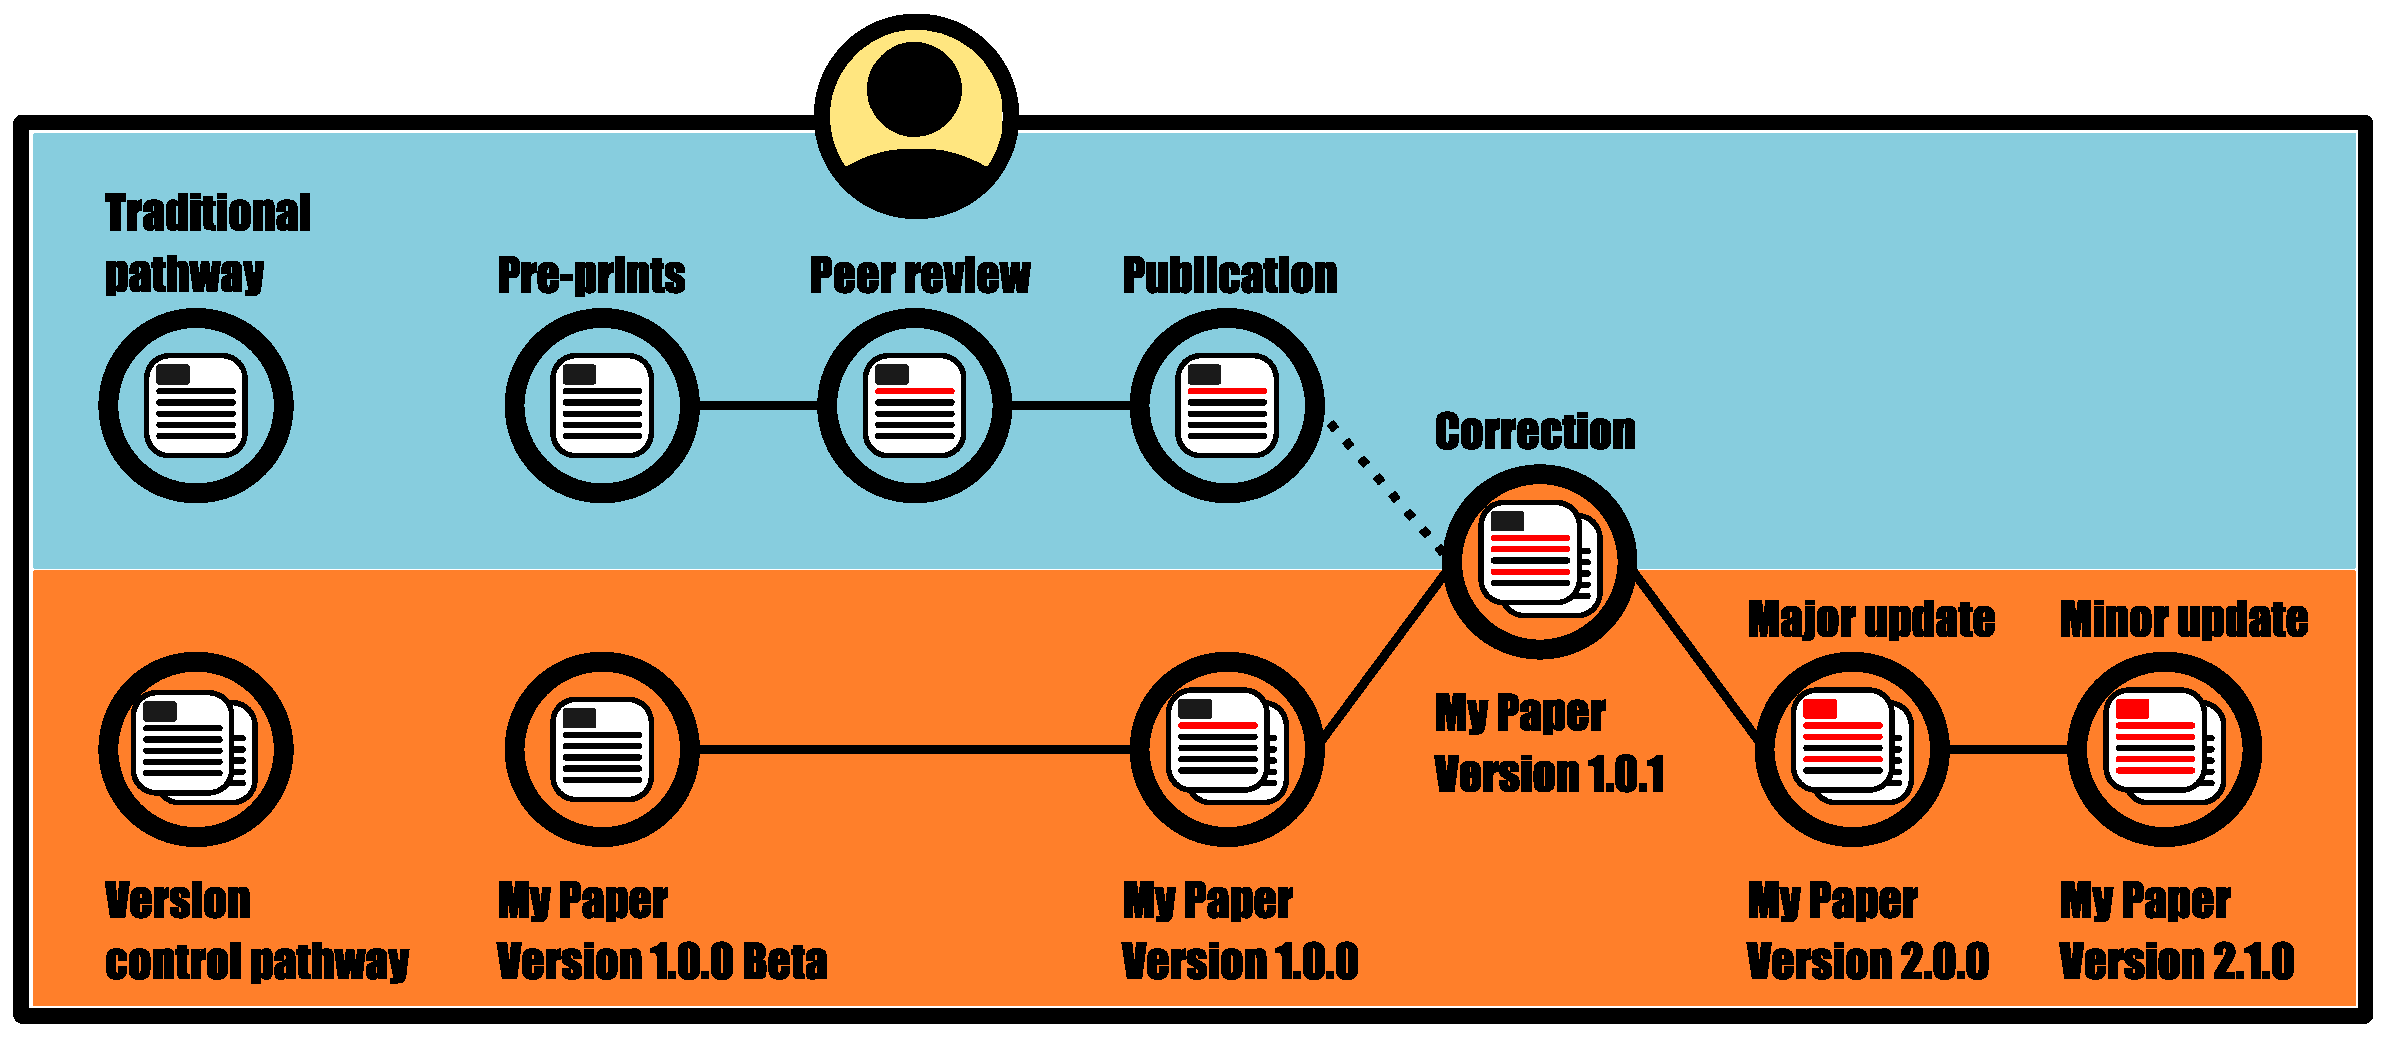
\includegraphics{./Figure/Figure1.pdf} Fig.1 - Graphical representation
of our proposed system that shows its relationship with the current
system. Our system deals with the barriers (dashed line) that are now
currently restricting authors from correcting their published work.

\hypertarget{benefits-and-potential-issues}{%
\subsection{Benefits and Potential
Issues}\label{benefits-and-potential-issues}}

There are some similar initiatives which speak to the scientific
dissatisfaction with the static publication model. For instance, Living
Reviews have version control but at the level of a review article, or
F1000research/ Evolving Papers which are editor-controlled forms of what
we have in mind. Then there is Manubot, which details a somewhat similar
approach and specifically requires GitHub to operate, but which mostly
targets the process pre-publication. (Himmelstein et al. 2019).

We believe there are multiple benefits to our proposed system. The
number one benefit is that it allows previously published work to be
amended and/or updated in a straightforward way because it is author
led. This takes out the middleman of the journals who do not need to be
involved at any step once the paper is published in its initial,
peer-reviewed state (see responses to Question 9 in the supplement).

We suspect that our relatively frictionless system would engender a
culture of correction including an awareness of correction as a
possibility (Teixeira da Silva and Al-Khatib 2021). Adhering to semantic
versioning would allow authors to have a natural flow if they use
preprints by referring to this version as the beta stage. Further, it
would offer plenty of grist for students to verify/update/correct the
work of their supervisor -- typically a principal investigator who may
have more time constraints. This would stand to benefit the students who
could point to tangible outputs from their own efforts on their CVs. It
would also empower authors to raise flags about their own work even if
they haven't yet had time to address them (cf.~the Loss-of-Confidence
Project (Rohrer et al. 2021)). Historical works that do not have an
internal link to GitHub could still be updated using this system by
establishing a page for the paper post hoc.

There are some potential issues with our proposal. For one, there is a
separation between the amendment and the journal, although this could
also be considered as a positive as argued before. The onus here is on
the authors to advertise any changes. The semantic versioning system
using the same title as the paper should help here in terms of search
engines turning up both. Further, as noted earlier, interested readers
could follow a GitHub repository of a paper so they are alerted to any
changes. Non open access journals could take issue with wholesale
replication of the publication outside of their website. Here authors
could discuss changes to specific sections of the paper that only those
with access to the paper could make sense of. Then there are questions
of what to do if the paper is so flawed that it needs to be retracted or
instances of malpractice. In this case we agree that contacting the
journal is best practice. Though here again, initial concerns could be
flagged early by the authors.

We argue that the concerns raised by people in our survey as well as our
own thoughts of potential shortcomings are not unique to this system.
Disagreement among co-authors, visibility of the amendment and
malpractice are some of the issues raised that pertain just as much to
the current system of corrections (Molckovsky, Vickers, and Tang 2011).
Indeed, we note that ours is an additional system, it allows for
immediate corrections, where authors can still go through the
established route if they desire.

\hypertarget{conclusions}{%
\subsection{Conclusions}\label{conclusions}}

Our findings add more weight to the view that the current system of
academic publication hinders science by disincentivising corrections and
amendments to published literature (Allison et al. 2016). A system of
version control, as we detail here, would offer numerous benefits to
what is an inherently dynamic and imperfect process of discovery
(Ioannidis 2005), all the while keeping the version of record. The
fundamentals to this system are already out there and simply require
buy-in from the community. Although it is not a perfect system, we
believe a constantly updating and updateable literature that is in the
hands of the authors better reflects the ideal of science. With this, we
can take another step towards a more robust and reliable scientific
literature and an improved working academic climate.

\hypertarget{ethics}{%
\subsection{Ethics}\label{ethics}}

Ethical clearance was granted by UCD's Human Research Ethics Committee -
Research Ethics Reference Number: LS-E-21-281-Amin-Kane.

\hypertarget{acknowledgements}{%
\subsection{Acknowledgements}\label{acknowledgements}}

Thanks to the Laboratory of Wildlife Ecology and Behaviour at UCD for
testing our survey and providing valuable feedback on the questions.

\hypertarget{open-science-statement}{%
\subsection{Open Science statement}\label{open-science-statement}}

Updates of this paper can be found following this link:
\url{https://github.com/kanead/Corrections}

\hypertarget{references}{%
\subsection*{References}\label{references}}
\addcontentsline{toc}{subsection}{References}

\hypertarget{refs}{}
\begin{CSLReferences}{1}{0}
\leavevmode\vadjust pre{\hypertarget{ref-allison2016reproducibility}{}}%
Allison, David B, Andrew W Brown, Brandon J George, and Kathryn A
Kaiser. 2016. {``Reproducibility: A Tragedy of Errors.''} \emph{Nature}
530 (7588): 27--29.

\leavevmode\vadjust pre{\hypertarget{ref-barbour2017amending}{}}%
Barbour, Virginia, Theodora Bloom, Jennifer Lin, and Elizabeth Moylan.
2017. {``Amending Published Articles: Time to Rethink Retractions and
Corrections?''} \emph{F1000Research} 6 (1960): 1960.

\leavevmode\vadjust pre{\hypertarget{ref-chawla2019lose}{}}%
Chawla, D. 2019. {``It's Okay to Lose Confidence in Your Previous
Research.''} \emph{Nature Index}.

\leavevmode\vadjust pre{\hypertarget{ref-conroy2020reveal}{}}%
Conroy, G. 2020. {``Scientists Reveal What They Learnt from Their
Biggest Mistakes.''} \emph{Nature Index}.

\leavevmode\vadjust pre{\hypertarget{ref-else2017likely}{}}%
Else, Holly. 2017. {``How Likely Are Academics to Confess to Errors in
Research?''} \emph{Times Higher Education}.

\leavevmode\vadjust pre{\hypertarget{ref-himmelstein2019open}{}}%
Himmelstein, Daniel S, Vincent Rubinetti, David R Slochower, Dongbo Hu,
Venkat S Malladi, Casey S Greene, and Anthony Gitter. 2019. {``Open
Collaborative Writing with Manubot.''} \emph{PLOS Computational Biology}
15 (6): e1007128.

\leavevmode\vadjust pre{\hypertarget{ref-ioannidis2005most}{}}%
Ioannidis, John PA. 2005. {``Why Most Published Research Findings Are
False.''} \emph{PLoS Medicine} 2 (8): e124.

\leavevmode\vadjust pre{\hypertarget{ref-kendall2019persistent}{}}%
Kendall, Bruce E, Masami Fujiwara, Jasmin Diaz-Lopez, Sandra Schneider,
Jakob Voigt, and Sören Wiesner. 2019. {``Persistent Problems in the
Construction of Matrix Population Models.''} \emph{Ecological Modelling}
406: 33--43.

\leavevmode\vadjust pre{\hypertarget{ref-molckovsky2011characterization}{}}%
Molckovsky, A, MM Vickers, and Patricia Tang. 2011. {``Characterization
of Published Errors in High-Impact Oncology Journals.''} \emph{Current
Oncology} 18 (1): 26--32.

\leavevmode\vadjust pre{\hypertarget{ref-o2021towards}{}}%
O'Dea, Rose E, Timothy H Parker, Yung En Chee, Antica Culina, Szymon M
Drobniak, David H Duncan, Fiona Fidler, et al. 2021. {``Towards Open,
Reliable, and Transparent Ecology and Evolutionary Biology.''} \emph{BMC
Biology} 19 (1): 1--5.

\leavevmode\vadjust pre{\hypertarget{ref-rohrer2021putting}{}}%
Rohrer, Julia M, Warren Tierney, Eric L Uhlmann, Lisa M DeBruine, Tom
Heyman, Benedict Jones, Stefan C Schmukle, et al. 2021. {``Putting the
Self in Self-Correction: Findings from the Loss-of-Confidence
Project.''} \emph{Perspectives on Psychological Science} 16 (6):
1255--69.

\leavevmode\vadjust pre{\hypertarget{ref-sandve2013ten}{}}%
Sandve, Geir Kjetil, Anton Nekrutenko, James Taylor, and Eivind Hovig.
2013. {``Ten Simple Rules for Reproducible Computational Research.''}
\emph{PLoS Computational Biology} 9 (10): e1003285.

\leavevmode\vadjust pre{\hypertarget{ref-teixeira2021ending}{}}%
Teixeira da Silva, Jaime A, and Aceil Al-Khatib. 2021. {``Ending the
Retraction Stigma: Encouraging the Reporting of Errors in the Biomedical
Record.''} \emph{Research Ethics} 17 (2): 251--59.

\leavevmode\vadjust pre{\hypertarget{ref-vuong2020limitations}{}}%
Vuong, Quan-Hoang. 2020. {``The Limitations of Retraction Notices and
the Heroic Acts of Authors Who Correct the Scholarly Record: An Analysis
of Retractions of Papers Published from 1975 to 2019.''} \emph{Learned
Publishing} 33 (2): 119--30.

\end{CSLReferences}

\end{document}
